\Chapter{Egy étterem, egy futár, egy kiszállítás esete}

\Section{A probléma megfogalmazása}

Ebben az esetben egy étterem található a városban, amelyből csak egy futár szállít ki mindig csak egy címre.
Bonyolultságát tekintve a legrövidebb utat kell megtalálni az úthálózat gráfjának két pontja között, feltételezve azt, hogy egy pontból a másikba nem feltétlenül lehet közvetlenül eljutni, csak más pontok érintésével. Ezáltal egy gráf élein kell végigmenni és közben keresni a legrövidebb hosszúságú utat. Az optimális út meghatározása után venni kell ezen út hosszúnak kétszeresét, mivel a futár a szállítást követően vissza kell, hogy térjen az étterembe.
A probléma szemléltetését \aref{fig:model1}. ábrán láthatjuk \cite{Diagrams.net}.

\begin{figure}[h!]
\centering
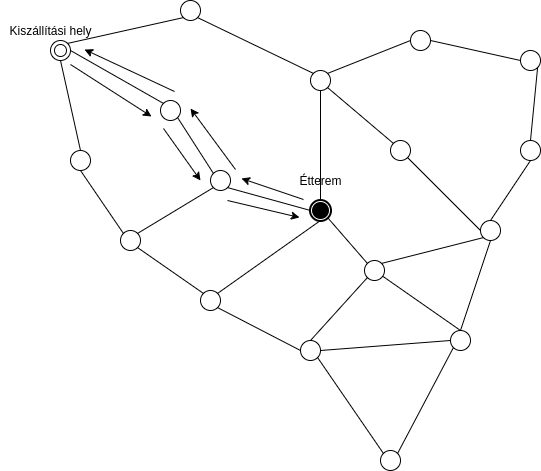
\includegraphics[scale=0.5]{images/Astar.png}
\caption{Egy étterem, egy futár, egy kiszállítás modellje}
\label{fig:model1}
\end{figure}

Két pont között a legrövidebb útvonal meghatározásához az $A^{*}$ algoritmus egy igen hatékony megoldást ad \cite{Astar}.
A következő szakaszban ennek részletezése következik.

\Section{A probléma megoldása}

Az $A^{*}$ algoritmusban a kiértékelő függvényünk egy heurisztikus függvény.
Egy iteratív algoritmusról van szó.
A fő ciklus minden iterációjánál az $A^{*}$-nak meg kell határoznia az általala kiterjesztendő utat.
A szakasz költségét és a célhoz érésnek költségét veszi figyelembe, így az $A^{*}$ meghatározza az $f(n) = g(n) + h(n)$ függvényt minimalizáló utat. Itt $n$-nel jelöljük a következő úton található csúcsot, ezáltal $g(n)$ a kezdőpontból $n$-ig tartó út költsége. A heurisztikus függvény $h(n)$-nel azonosítható, ez pedig nem más mint az $n$-től a célig vezető legkisebb költségű út költségének becslése.

Az algoritmus a meglátogatott pontokat tárolja, így nagy méretű problémák esetében nagy lehet a memóriaigénye is.
Az esetünkben vizsgált problémák esetében ebből szerencsére nem jelentett problémát. 

\Section{A megoldás implementálása}

Érdemes az aktuálisan megoldandó feladat leírásához egy olyan formalizmust használni, amelyik egyszerűen adaptálható lehet a későbbiekben a valóságban is előforduló esetekhez.
Abból indulhatunk ki, hogy a város úthálózatának megadását a térkép ismeretében néhány kézenfekvő átalakítási lépéssel jó lenne megoldani.
Természetesen adódik, hogy így az úthálózat térképe egy kép legyen, amelyen be vannak jelölve azok az utak, amiken a futár haladhat.
Mivel a kép lehet színes is, ezért egyúttal az éttermek és a kiszállítási helyek megkülönböztetésére is lehetőség adódik.

A térkép betöltéséhez az OpenCV függvénykönyvtárat használhatjuk \cite{PythonOpenCV}.
Ehhez az alábbi kódsor szükséges.
\begin{python}
import cv2
\end{python}

Definiáljunk egy \texttt{Node} nevű osztályt, amelynek inicializálása a következőképpen történik \cite{Python}.
\begin{python}
def __init__(self, parent=None, position=None):
    self.parent = parent
    self.position = position

    self.g = 0
    self.h = 0
    self.f = 0
\end{python}
Ebben \texttt{g}-vel jelöljük a kezdőpontot, \texttt{h}-val a célt és \texttt{f}-el pedig a költséget.

A következő definiciók nélkülözhetetlenek a pontok összehasonlítási folyamatában.

\begin{python}
def __eq__(self, other):
    return self.position == other.position

def __hash__(self):
    return hash(self.position)
\end{python}

Az $A^{*}$ algoritmus ezek segítségével a következőképpen írható le.
Létrehozunk két csomópontot, úgy mint a \texttt{startNode} kezdő- és \texttt{endNode} végpontot.
\begin{python}
startNode = Node(None, start)
startNode.g = startNode.h = startNode.f = 0
endNode = Node(None, end)
endNode.g = endNode.h = endNode.f = 0
\end{python}
Ezt követően inicializálunk két listát, melyek a már látogatott pontokat tartják majd nyilván (nyitott és zárt lista).
\begin{python}
openList = []
closedList = set()
\end{python}
Megadjuk a kezdő csomópontot azáltal, hogy a nyitott listába rakjuk.
\begin{python}
openList.append(startNode)
\end{python}
Ezt kövezően ciklust indítunk, ami addig tart, amíg el nem éri a végpontot.
\begin{python}
while len(openList) > 0:
\end{python}
A cikluson belül a következőképpen határozható meg a jelenlegi csomópont.
\begin{python}
currentNode = openList[0]
currentIndex = 0
for index, item in enumerate(openList):
   if item.f < currentNode.f:
       currentNode = item
       currentIndex = index
\end{python}      
A nyitott listából a zárt listába a következőképp rakjuk át az adott elemet:
\begin{python}
openList.pop(currentIndex)
closedList.add(currentNode)
\end{python}
A célhoz vezető út meghatározása a következőképpen zajlik.
\begin{python}
if currentNode == endNode:
    path = []
    current = currentNode
    while current is not None:
        path.append(current.position)
        current = current.parent
    return path[::-1]
\end{python}

Az út meghatározásában nagy szerepet játszik a navigáció; észak, dél, kelet és nyugat irányban tudunk elindulni, köztes irányok nincsennek. Meg kell hatázozni a csomópont pozicióját. Ezt követően egyértelművé kell hogy váljon, hogy közvetlenül el lehet-e érni azt. Le kell ellenőrizni, hogy az adott pont tényleg út-e. Mindezek után hozunk létre egy új csomópontot amit az után hozzáadunk az új lehetséges úthoz.

Mivel a probléma nagyon hasonló egy labirintusban való útvonal kereséséhez, ezért a térképet az algoritmus szempontjából \texttt{maze} változóként kezeljük.
\begin{python}
newWay = []                
for newPosition in [(0, -1), (0, 1), (-1, 0), (1, 0)]:
    nodePosition = (currentNode.position[0] + newPosition[0], 
            		currentNode.position[1] + newPosition[1])

    if nodePosition[0] > (len(maze) - 1) or 
    nodePosition[0] < 0 or 
    nodePosition[1] > (len(maze[len(maze)-1]) -1) or 
    nodePosition[1] < 0:
        continue

    if maze[nodePosition[0]][nodePosition[1]] != 0:
        continue

    newNode = Node(currentNode, nodePosition)
    
    newWay.append(newNode)
\end{python}

Az algoritmus utolsó lépéseként megvizsgáljuk ezen lehetséges utakat, kiértékeljük a már fentebb említett \texttt{f}, \texttt{g} és \texttt{h} értékeket, majd ezek által kiválasztjuk a legkedvezőbbet.
\begin{python}
for way in newWay:

    if way in closedList:
        continue

    way.g = currentNode.g + 1
    way.h = ((way.position[0] - endNode.position[0]) ** 2) + 
    		((way.position[1] - endNode.position[1]) ** 2)
    way.f = way.g + way.h

    for openNode in openList:
        if way == openNode and way.g > openNode.g:
            continue

    openList.append(way)
\end{python}

Az implementációs rész elején említett \texttt{cv2} csomag a következők okok miatt szükséges.
Adott egy kép, ami fekete $(0, 0, 0)$, fehér $(255, 255, 255)$, egy piros $(0 ,0, 255)$ és egy kék $(255,0,0)$ színű pontokból tevődik össze (ahol a hármasokban az értékek a kék, zöld és piros csatornák intenzitását jelentik $[0, 255]$ egészes intervallumon). A fekete jelképezi a járhatatlan utat. Fehér színnel van jelölve a járható út. A piros szín mutatja meg a rendelési helyet, míg a kék az éttermet szimbolizálja. Az ilyen formában rendelkezésre álló kép feldolgozáshoz a következők inicializálások szükségesek.

\begin{python}
img = cv2.imread("AStarProblem.bmp")
height, width, channels = img.shape

blue =  "[255   0   0]"
red =   "[  0   0 255]"
black = "[  0   0   0]"
white = "[255 255 255]"

mazeHelp = []
maze = []
\end{python}

A kép minden pontján áthaladva egy kettős ciklussal meghatározható a pixel pontos színe. Ebből egy tömböt kreálva elkészül az $A^{*}$ algoritmushoz felhasználható térkép. Futtatva az algoritmust az optimális utat kiszínezi sárga színnel az étterem és a kiszállítás helye között.

\begin{python}
for i in range(width):
    for j in range(height):
        if (str(img[i, j]) in white):
            mazeHelp.append(0)
        if (str(img[i, j]) in black):
            mazeHelp.append(1)
        if (str(img[i, j]) in red):
            mazeHelp.append(0)
            start = (i, j)
        if (str(img[i, j]) in blue):
            mazeHelp.append(0)
            end = (i, j)
    maze.append(mazeHelp)
    mazeHelp = []
path = aStar(maze, start, end)

for k in path:
    img[k] = [0, 255, 255]
cv2.imwrite('AStarResult.bmp', img)
\end{python}

\Section{A megoldás tesztelése}

A megoldás teszteléséhez nélkülözhetetlen egy BMP kép. A program megfelelő futásá\-hoz azt feltételezzük, hogy a kép hosszúsága és szélessége megegyezik. A fehér színnel kell kitelteni a járható utat, feketével a járhatatlant. Kék szín kell, hogy jelezze az éttermet, piros pedig a kiszállítási helyet. Amennyiben van lehetséges út az utóbbi két pont között, az alakalmazás megtalálja, valamint ha több út is tartozik hozzá, akkor a lehető legrövidebbet adja válaszul. Az eredmény egy képet generál, amin sárgával van feltüntetve az optimális út.

Egy kézzel rajzolt, várostérkép \aref{fig:model1problem}. ábrán látható formában néz ki.

\begin{figure}[h!]
\centering
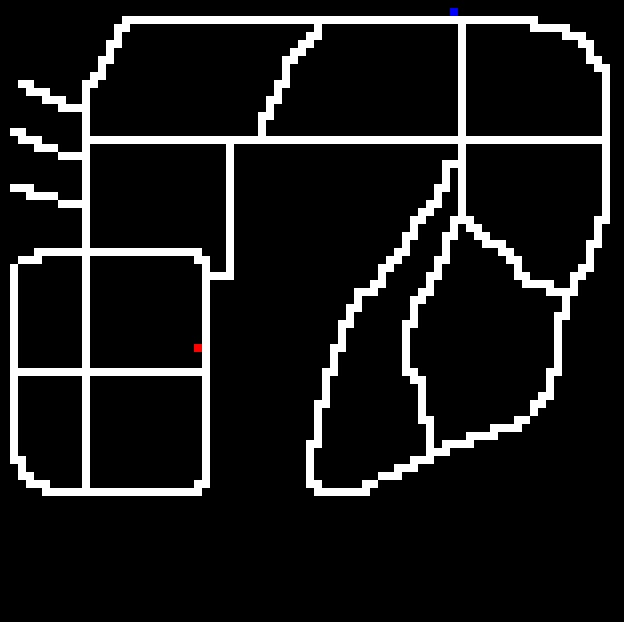
\includegraphics[scale=0.6]{images/AStarProblem.jpg}
\caption{A teszteléshez használt térkép}
\label{fig:model1problem}
\end{figure}

A megoldást felhasználva \aref{fig:model1result}. ábrán látható képet kapjuk.

\begin{figure}[h!]
\centering
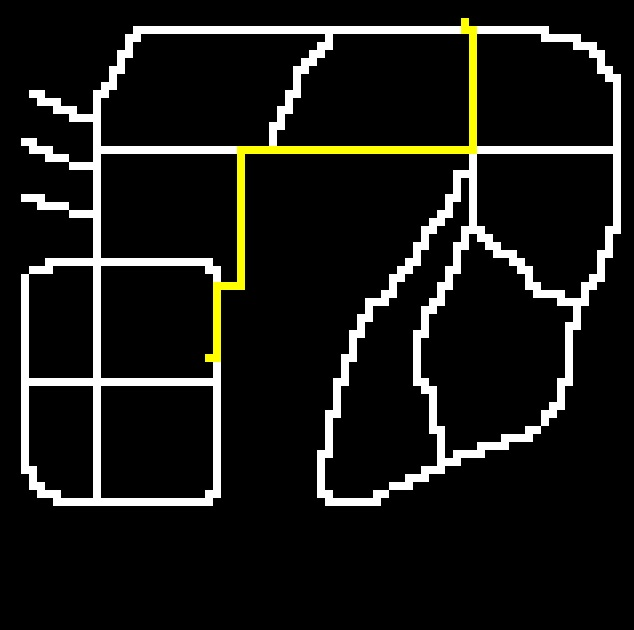
\includegraphics[scale=0.6]{images/AStarResult.jpg}
\caption{Az eredményül kapott útvonal}
\label{fig:model1result}
\end{figure}

A kép kíválóan szemlélteti, hogy optimális utat adott eredményül, ezáltal az algoritmus felhasználható az adott feladathoz.
